\documentclass{report}
\usepackage[utf8]{inputenc}
\usepackage[T1]{fontenc}
\usepackage[frenchb]{babel}
\usepackage[pdftex]{graphicx}
\usepackage{amsthm}
\usepackage{amsmath}
\usepackage{amssymb}
\usepackage{mathrsfs}

\usepackage{float}
\usepackage[colorlinks=true, allcolors=blue]{hyperref}

\title{TIVA-TP6}  
\begin{document}
\maketitle
\section*{Visualisation des Ondelettes 2D}
\subsection*{Question 1}
Familles d'ondelettes: Haar, Daubechies, Beylkin, Coiflet, Symmlet, Vaidyanathan, Battle.
\begin{figure}[H]
\begin{center}
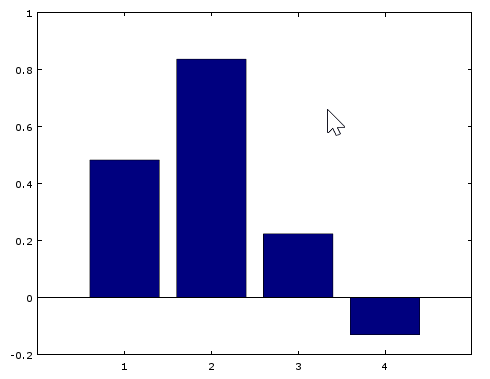
\includegraphics{Daubechies4.png}
\end{center}
\caption{Daubechies 4}
\end{figure}

\begin{figure}[H]
\begin{center}
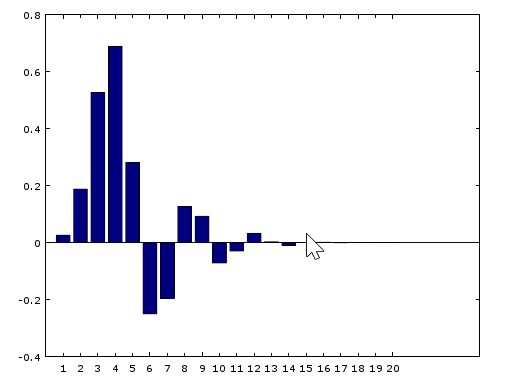
\includegraphics{Daubechies20.png}
\end{center}
\caption{Daubechies 20}
\end{figure}

\begin{figure}[H]
\begin{center}
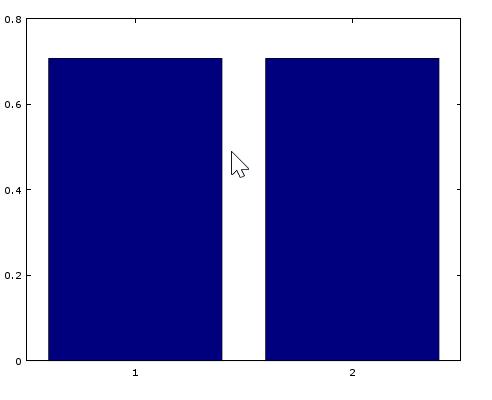
\includegraphics{Haar.png}
\end{center}
\caption{Haar}
\end{figure}

\subsection*{Question2}

\subsection*{Question 3}
Il y aura dans $W$ des coefficients associés à $\phi_{j, (n_1, n_2)}$ pour $j \in \{0, ..., 4\}$, et des coefficients associés à $\psi^k_{j, (n_1, n_2)}$ pour $j\in \{1, ..., 4\}$.\\
Pour $k$ et $j$ fixés, $n_1$ et $n_2$ varient dans $[0,\ 256/(2^{j+1})]$.\\
Le coefficient associé à $\psi^k_{j,(n_1,n_2)}$ se situe à: 
\begin{eqnarray*}
(m_1, m_2) = 
\left\{
\begin{array}{r c l}
 (n_1, 2^{(L-j)}+n_2), &\mbox{ si } k=1\\
 (2^{(L-j)}+n_1, n_2), &\mbox{ si } k=2\\
 (2^{(L-j)}+n_1, 2^{(L-j)}+n_2), &\mbox{ si } k=3 
 \end{array}
 \right.
 \end{eqnarray*}
\subsection*{Question 4}
On crée une matrice $\tilde{W}$ où tous les coefficients sont nuls sauf celui en $(m_1, m_2)$, coordonnées explicitées juste au dessus, qui vaut $1$, puis on fait la transformée inverse de cette matrice.

\subsection*{Question 5}
Si seul le coeeficient de coordonnées $(m_1, m_2)$ est non nul et égal à un, alors:
\begin{itemize}
	\item
	Si $m_1 \leq 2^{(8-L)}$ et $m_2\leq 2^{(8-L)}$, alors la transformée inverse de $W$ sera simplement la visualisation de l'ondelette père $\phi_{L, (m_1, m_2)}$;
	\item S
	Sinon, la transformée inverse de $W$ est la visualisation de l'ondelette mère $\psi^k_{j, (n_1, n_2)}$  avec la relation entre $(k, j, n_1, n_2)$ et $(m_1, m_2)$ précédamment établie.\\
\end{itemize}
En fait si l'on souhaite obtenir $phi_{j, (n_1, n_2)}$ avec $j<L$, il nous suffit de constater que comme:
\begin{eqnarray*}
\phi_{j, (n_1, n_2)} &=& \phi_{j, n_1}\phi_{j, n_2}\\
\psi^1_{j, (n_1, n_2)} &=& \phi_{j, n_1}\psi_{j, n_2}\\
\psi^2_{j, (n_1, n_2)} &=& \psi_{j, n_1}\phi_{j, n_2}\\
\psi^2_{j,(n_1, n_2)} &=& \psi_{j, n_1}\psi_{j, n_2}
\end{eqnarray*}
Alors on obtient:
\begin{eqnarray*}
\phi_{j, (n_1, n_2)} &=& \frac{\psi^1_{j, (n_1, n_2)}\psi^2_{j, (n_1, n_2)}}{\psi^3_{j, (n_1, n_2)}}
\end{eqnarray*} 
D'où pour obtenir une image de $\phi_{j, (n_1, n_2)}$ (si $j<L$, sinon c'est immédiat), il suffit de créer les matrices $W_1$, $W_2$ et $W_3$ qui ont respectivement tous leurs coefficients nuls sauf un qui vaut 1 aux coordonnées qui correspondent  à $(k=1, j, n_1, n_2)$, $(k=2, j, n_1, n_2)$ et $(k=3, j, n_1, n_2)$ d'après la relation écrite plus haut.\\
Puis on effectue le calcul:
\begin{eqnarray*}
Im &=& \frac{IWT(W_1)\cdot IWT(W_2)}{ITW(W_3)}
\end{eqnarray*}
où $Im$ est notre image résultat.
\end{document}